\documentclass[aspectratio=169]{beamer}
\usepackage[utf8]{inputenc}
%\usepackage[authordate,backend=biber,natbib]{biblatex-chicago}
%\usepackage{booktabs}
%\addbibresource{growthreferences.bib}

%\usepackage{utopia} %font utopia imported

\usetheme{Madrid}
\usecolortheme{beaver}

%------------------------------------------------------------
%This block of code defines the information to appear in the
%Title page
\title[Autor, Dorn, and Hanson (2016)] %optional
{The China Shock: Learning from Labor Market Adjustment to Large Changes in Trade}

\subtitle{David Autor, David Dorn, and Gordon Hanson, \emph{Annual Review of Economics}, 2016}

\author [Hauk] % (optional)
{William~R.~Hauk,~Jr.} %\inst{1} %\and J.~Doe\inst{2}} 

\institute[UofSC] % (optional)
{
  %\inst{1}%
  Darla Moore School of Business\\
  University of South Carolina
  %\and
  %\inst{2}%
  %Faculty of Chemistry\\
  %Very Famous University
}

\date[ECON 860, Fall 2021] % (optional)
{ECON 860 -- International Trade Theory\\Fall 2021}

\logo{
\includegraphics[height=1cm]{UofSC_Monogram_Stack_CMYK_G.jpg}}

%End of title page configuration block

%---------------------------------------------------------

\AtBeginSection[]
{
  \begin{frame}
    \frametitle{Table of Contents}
    \tableofcontents[currentsection,hideallsubsections]
  \end{frame}
}

%------------------------------------------------------------

\begin{document}

%The next statement creates the title page.
\frame{\titlepage}

%-------------------------------------------------------------

\section{Introduction}

%-------------------------------------------------------------

\begin{frame}{Introduction}

\begin{itemize}
    \item<1-> The standard undergraduate textbook tells us that trade is good for a country’s overall welfare.  There are distributional effects, but the gains to the winners are sufficient to compensate the losers.
    \item<2-> Strong consensus in economics towards free trade.  Even as evidence emerged in 1980s and 1990s of gaps between skilled and unskilled workers, this was explained empirically as more of a technology shock than a trade shock.
    \item<3-> Even when workers did lose their jobs due to trade, they should be able to reallocate easily to other industries.  Short-to-medium run gains from trade should be positive.
\end{itemize}
    
\end{frame}

%-------------------------------------------------------------

\begin{frame}{Figure 1}

\begin{figure}
    \centering
    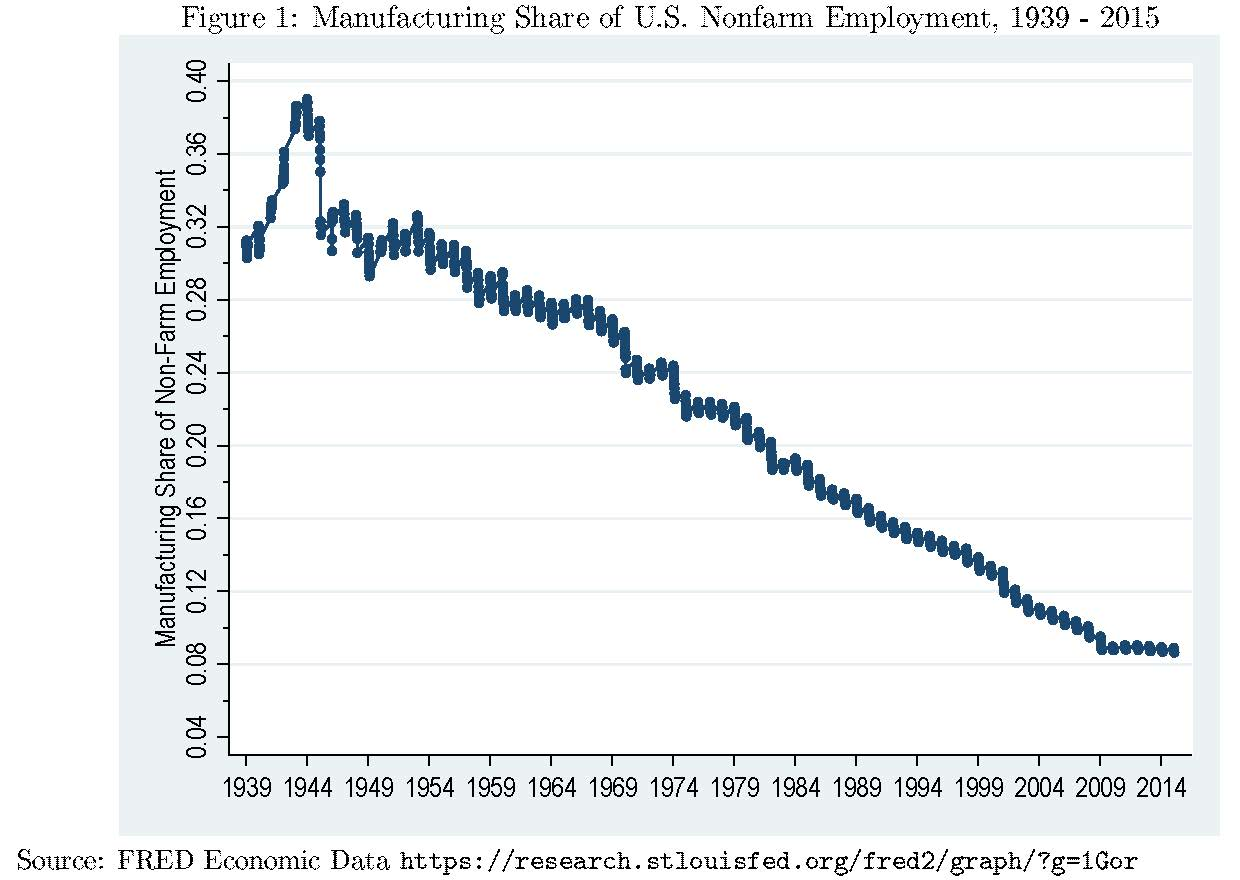
\includegraphics[scale=0.6]{AutorDornHansonFig1.jpg}
    \label{fig:fig1}
\end{figure}
    
\end{frame}

%-------------------------------------------------------------

\section{China's Rise}

%-------------------------------------------------------------

\begin{frame}{Rise of Chinese Manufacturing}

\begin{itemize}
    \item<1-> Rise of China has challenged the consensus on trade and wages.  Distributional effects (theory has recognized) and adjustment costs (theory has tended to downplay) have been relatively large.
    \item<2->  Many pundits were pessimistic about China’s chances as recently as late 1980s due to turmoil from Tiananmen Square incident
    \item<3-> Reformers gained upper hand in early 1990s, and manufacturing activity in China exploded, especially in Special Economic Zones on the east coast.  Number of SEZs increased from 20 in 1991 to 150 in 2010.
    \item<4-> Chinese share of world manufacturing exports grew from 2.3\% in 1991 to 18.8\% in 2013.  
\end{itemize}
    
\end{frame}

%-------------------------------------------------------------

\begin{frame}{Figure 2}

\begin{figure}
    \centering
    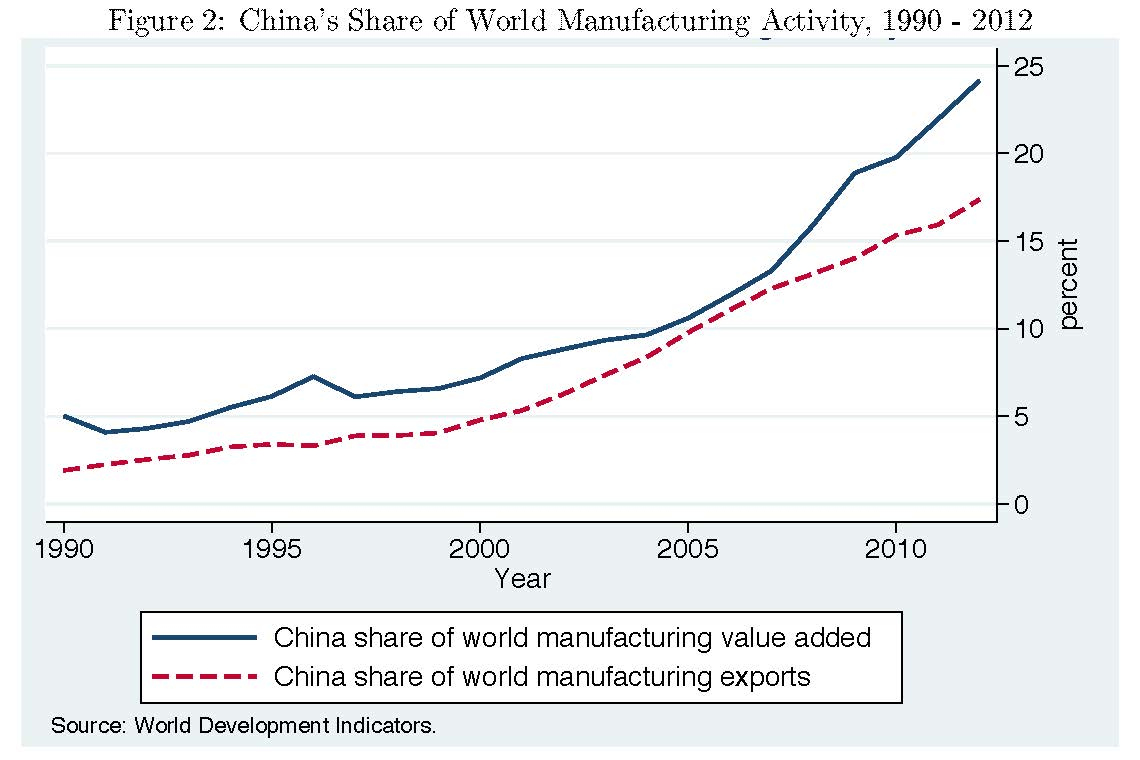
\includegraphics[scale=0.7]{AutorDornHansonFig2.jpg}
    \label{fig:fig2}
\end{figure}
    
\end{frame}

%-------------------------------------------------------------

\subsection{Making Use of Trade Shocks}

%-------------------------------------------------------------

\begin{frame}{The China ``Shock"}

\begin{itemize}
    \item<1-> Autor, Dorn, and Hanson make the argument that the Chinese transition to a manufacturing exporter owes more to internal political and economic issues in China than the global economy.  Thus, its growth is plausibly exogenous.
    \item<2-> The rise of China is importance both because of its magnitude and the relative paucity of natural experiments in international trade.  (E.g. NAFTA was caused by foreign investment as much as it caused foreign investment.)
\end{itemize}
    
\end{frame}

%-------------------------------------------------------------

\begin{frame}{Why We Should Study China}

Three features of China’s experience make it worthy of detailed study:

\begin{itemize}
    \item<1-> Unexpected nature of China’s export growth caught many people by surprise.
    \item<2-> China’s relative degree of isolation under Mao, which created a lot of opportunity for China to catch up.
    \item<3->  Manufacturing was at the heart of its economic turn-around, as opposed to raw materials – large positive supply shock in manufacturing and large demand shock for raw materials.
\end{itemize}
    
\end{frame}

%-------------------------------------------------------------

\subsection{The Global Factory}

%-------------------------------------------------------------

\begin{frame}{Figure 3.A}

\begin{figure}
    \centering
    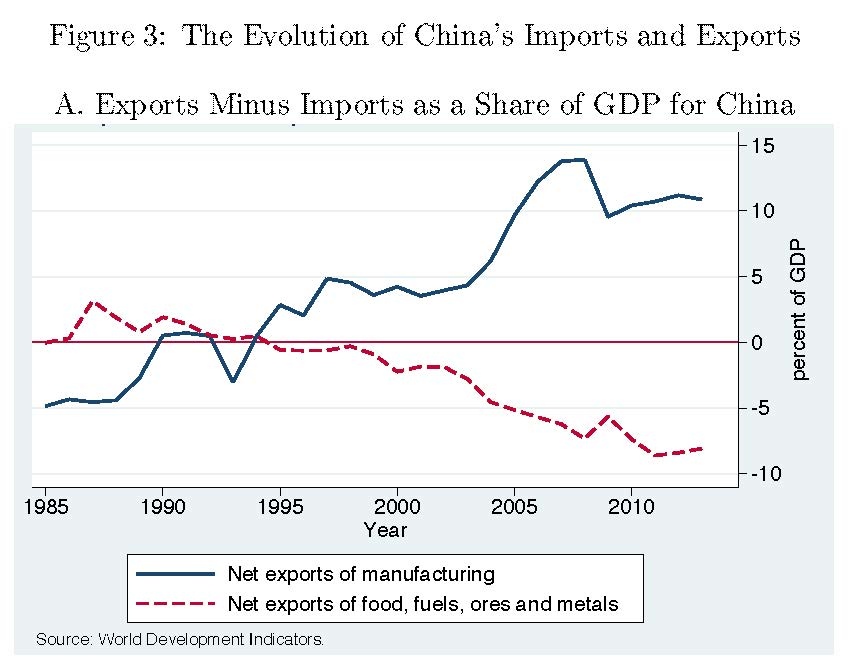
\includegraphics[scale=0.8]{AutorDornHansonFig3a.jpg}
    \label{fig:fig3a}
\end{figure}
    
\end{frame}

%-------------------------------------------------------------

\begin{frame}{Figure 3.B}

\begin{figure}
    \centering
    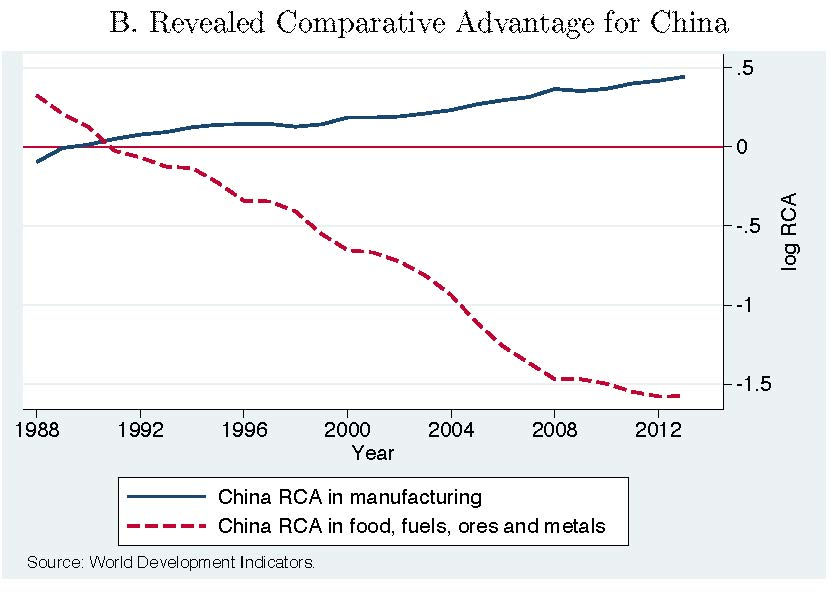
\includegraphics[scale=0.85]{AutorDornHansonFig3b.jpg}
    \label{fig:fig3b}
\end{figure}
    
\end{frame}

%-------------------------------------------------------------

\begin{frame}{The Global Factory}

\begin{itemize}
    \item<1-> China probably had a long-standing comparative advantage in manufacturing, but it remained latent during the Maoist era.  Strength only emerged in late 1980s.
    \item<2-> In 1992, China moved from a comparative disadvantage to comparative advantage in manufactures, and from a comparative advantage to disadvantage in primary products.
    \item<3-> However, as noted by Figure 4, China’s net import penetration varied substantially across industries.  Because of this variation, U.S. industries, and the regions in which they locate, vary widely in their exposure to import competition from China.
\end{itemize}
    
\end{frame}

%-------------------------------------------------------------

\begin{frame}{Figure 4}

\begin{figure}
    \centering
    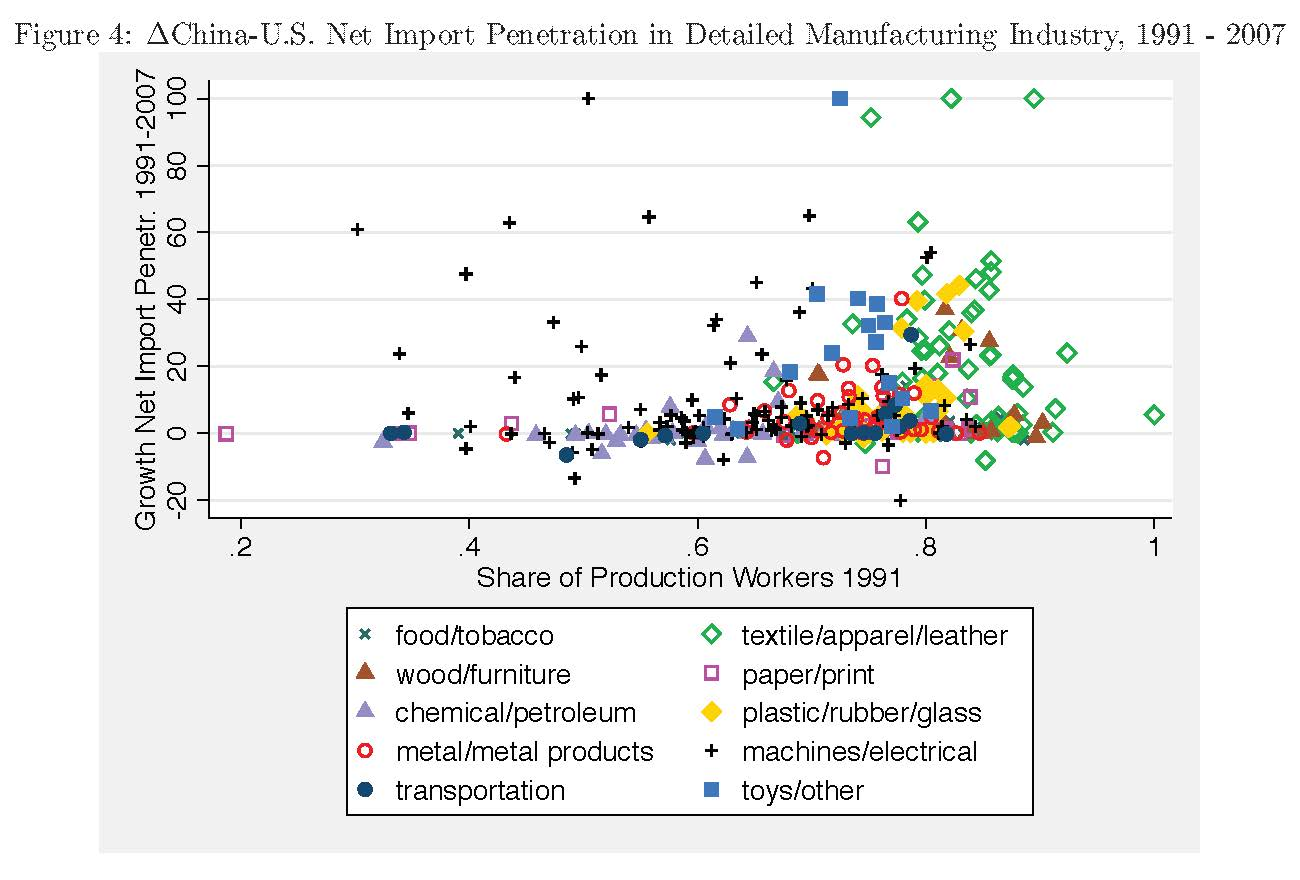
\includegraphics[scale=0.6]{AutorDornHansonFig4.jpg}
    \label{fig:fig4}
\end{figure}
    
\end{frame}

%-------------------------------------------------------------

\begin{frame}{WTO Accession 2001}

\begin{itemize}
    \item<1-> Chinese manufacturing accelerated after WTO accession in 2001.  At the same time, China had a huge surge in manufacturing productivity – pace of growth was about 8\% a year between 1998 and 2007.
    \item<2-> WTO membership meant that China liberalized many state-owned manufacturing firms and got steadier access to raw materials, helping productivity growth.
\end{itemize}
    
\end{frame}

%-------------------------------------------------------------

\subsection{The Global Macroeconomic Context}

%-------------------------------------------------------------

\begin{frame}{The Global Macroeconomic Context}

\begin{itemize}
    \item<1-> During this time period, China’s trade surplus increased substantially, while the U.S.'s worsened.
    \item<2-> Because these are the two largest economies in the world and the U.S. dollar functions as a global reserve currency, China’s trade surplus resulted in large purchases of dollar-denominated assets.
    \item<3-> Trade imbalances complicate the standard trade model.  Under balanced trade, U.S. workers shift from import-competing to export-oriented industries.
    \item<4-> With a large trade deficit, workers in import competing industries have to leave the traded goods sector and possibly the workforce entirely.
    \item<5-> At some point in the future, Chinese savings would fall, consumption would rise, and the trade flows would go in the other direction.
\end{itemize}
    
\end{frame}

%-------------------------------------------------------------

\begin{frame}{Figure 5}

\begin{figure}
    \centering
    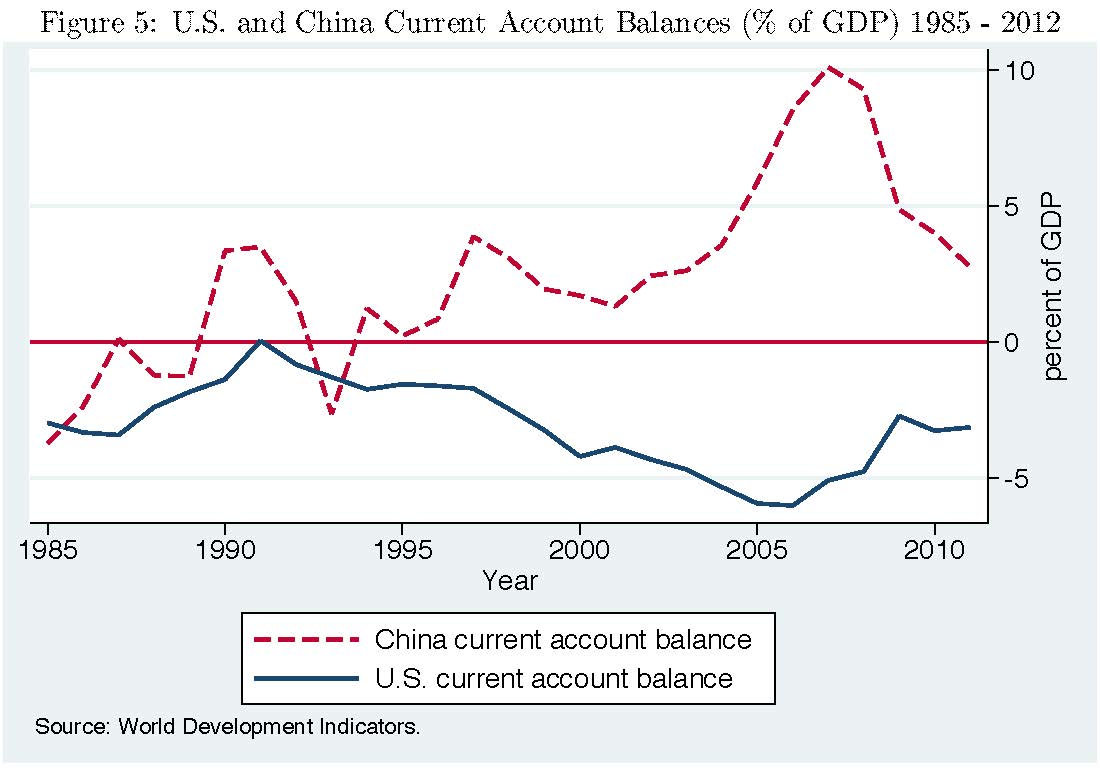
\includegraphics[scale=0.65]{AutorDornHansonFig5.jpg}
    \label{fig:fig5}
\end{figure}
    
\end{frame}

%-------------------------------------------------------------

\section{Theory}

%-------------------------------------------------------------

\begin{frame}{Theory}

\begin{itemize}
    \item<1-> Standard H-O model predicts a link between trade shocks and changes in factor returns, but this model has some shortcomings, which we have discussed previously.
    \item<2-> More recent work focuses on heterogeneous firms (e.g. Melitz (2003)).  Focus has been on the various margins through which firms adjust to trade shocks.
    \item<3-> Model proposed in this paper follows a trend of incorporating gravity-type structures, which allows for tractable descriptions of labor mobility between regions or industries.
    \item<4-> If there are frictions to worker mobility, then there are potentially several margins through which trade shocks could affect labor markets.
\end{itemize}
    
\end{frame}

%-------------------------------------------------------------

\subsection{A Bare Bones Model}

%-------------------------------------------------------------

\begin{frame}{A Bare Bones Model}

\begin{itemize}
    \item<1-> Model contains a single labor-market friction – imperfect labor mobility within the country.  Contrary to many other models, but perhaps better in tune with data.
    \item<2-> Begin with an assumption of complete geographic labor immobility.  Variation in regional exposure to foreign competition comes from differences in regional industry specializations.
\end{itemize}
    
\end{frame}

%-------------------------------------------------------------

\begin{frame}{Gravity-Like Trade}

Trade has a gravity-type structure – total demand by the U.S. aggregate economy for traded output produced in U.S. region $ i $ is:

\begin{equation}
    X_{i} = \sum_{k}\frac{A_{i,k} \tau_{i,k}^{-\theta}}{\Phi_k} E_{k}
    \label{eq:Xi}
\end{equation}

where $ A_{i,k} $ is the production capacity of industry $ k $ in region $ i $, $ \tau_{i,k} $ is an iceberg transportation cost to ship goods from region $ i $ in industry $ k $ to the U.S. market, $ \theta $ is the trade-cost elasticity, $ E_{k} $ is aggregate U.S. expenditure on industry $ k $, and $ \Phi_k = \sum_{i'} A_{i'} \tau_{i',k}^{-\theta} $ is a competitiveness index for the U.S. market in industry $ k $.
    
\end{frame}

%-------------------------------------------------------------

\begin{frame}{Change in Regional Output}

If there is a change in traded output in regions that supply the U.S., we can derive the impact on region i by totally differentiating equation (\ref{eq:Xi}):

\begin{equation}
    \hat{X}_{i} = \sum_{k} \phi_{i,k} \hat{E}_{k} - \theta \hat{w}_{i} + \sum_{k} \phi_{i,k} \hat{A}_{k} + \sum_{k} \phi_{i,k} \sum_{i' \neq c} \rho_{i',k} \hat{A}_{i',k} - \sum_{k} \phi_{i,k} \rho_{c,k} \hat{A}_{c,k}
    \label{eq:xihat}
\end{equation}

where $ c $ indexes China, $ \phi_{i,k} = \frac{X_{i,k}}{X_{i}} $ is the share of industry $ k $ in region $ i $’s total sales to the U.S. market, and $ \rho_{i,k} = X_{i,k} E_{k} $ is the share of region $ i $ in total U.S. expenditure on industry $ k $.  Also, assume that $ \hat{A}_{i,k} = \hat{A}_{k} - \theta \hat{w}_{i} $ (i.e. local productivity changes are reflected in national productivity changes and local wage changes). 
    
\end{frame}

%-------------------------------------------------------------

\begin{frame}{The China Shock}

\begin{itemize}
    \item<1-> We are primarily interested in the last part of equation (\ref{eq:xihat}), which captures the growth of China’s productive capacity on traded output in U.S. region $ i $.  Rewrite this as:
    \begin{equation}
        \sum_{k} \phi_{i,k} \rho_{c,k} \hat{A}_{c,k} = \sum_{k} \phi_{i,k} \left[ \frac{X_{c,k} \hat{A}_{c,k}}{E_{k}} \right]
        \label{eq:Chinashock}
    \end{equation}
    which is the weighted average exposure of region $ i $ to changes in U.S. industry import penetration mandated by changes in Chinese production capabilities.
    \item<2-> Because weights $ \phi_{i,k} $ vary across regions of the U.S., the exposure to Chinese traded goods varies across U.S. regions.
\end{itemize}
    
\end{frame}

%-------------------------------------------------------------

\subsection{Identifying the Reduced-Form Impact of the China Trade Shock}

%-------------------------------------------------------------

\begin{frame}{Identifying the Reduced-Form Impact of the China Trade Shock}

\begin{itemize}
    \item<1-> Estimating the impact of the trade shock in equation (\ref{eq:Chinashock}) requires that we control for confounding factors.  Fortunately, these factors are identified in equation (\ref{eq:xihat}).
    \item<2-> The first term in equation (\ref{eq:Xi}) is $ \sum_{k} \phi_{i,k} \hat{E}_{k} $, which is the regional exposure to U.S. industry demand shocks.  Reduced form regressions of regional outcomes on regional trade exposure might be contaminated by U.S. product demand shocks.
    \item<3-> Following Autor, Dorn, and Hanson (2013), this paper instruments for the growth in U.S. imports from China with the growth in Chinese imports in other high-income markets.
\end{itemize}
    
\end{frame}

%-------------------------------------------------------------

\begin{frame}{Table 1}

\begin{figure}
    \centering
    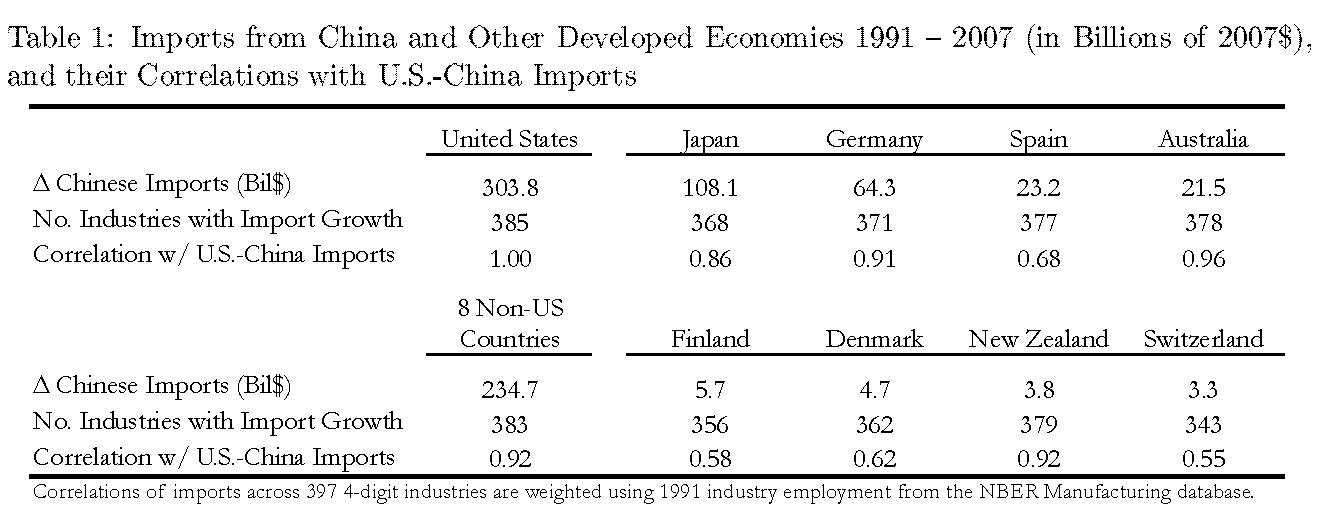
\includegraphics[scale=0.82]{AutorDornHansonTable1.jpg}
    \label{fig:Tab1}
\end{figure}
    
\end{frame}

%-------------------------------------------------------------

\begin{frame}{Instrumental Variables Strategy}

\begin{itemize}
    \item<1-> Table 1 documents the instrumental variables strategy.  Several other countries have a high correlation with the U.S. in terms of their growth in Chinese imports.
    \item<2-> There is a concern that demand changes might be correlated across high-income countries.
    \item<3-> Autor, Dorn, and Hanson (2013) also used a gravity-based strategy that used Chinese changes in revealed comparative advantage as an instrument (eliminating differences based on import demand in the purchasing country).
    \item<4-> Results did not change much, so they believe that it is not a major concern.
\end{itemize}
    
\end{frame}

%-------------------------------------------------------------

\begin{frame}{Wage Changes from Shocks}

\begin{itemize}
    \item<1-> The second term in equation (\ref{eq:xihat}) is $ \theta \hat{w}_{i} $, the endogenous change in wages in region i from trade shocks.
    \item<2-> One can estimate equation (\ref{eq:xihat}) without this term, in which case the reduced form result captures the effect on region i directly through changes in output, or indirectly through wages.
    \item<3-> Or, one can use $ \hat{w}_{i} $ as a dependent variable in a regression.
\end{itemize}
    
\end{frame}

%-------------------------------------------------------------

\begin{frame}{Change in National Industry Productivity}

\begin{itemize}
    \item<1-> The third term in equation (\ref{eq:Xi}) is $ \sum_{k} \phi_{i,k} \hat{A}_{k} $ which captures the exposure of region $ i $ to changes in national industry productivity.
    \item<2-> Autor, Dorn, and Hanson (2013, 2015) note that there is near zero correlation between technological change and exposure to trade with China across U.S. local labor markets.
    \item<3->  So there is little to no omitted variables bias from excluding this.
\end{itemize}
    
\end{frame}

%-------------------------------------------------------------

\begin{frame}{Production Capacity in Other Countries}

\begin{itemize}
    \item<1-> The fourth term in equation (\ref{eq:xihat}) is $ \sum_{k} \phi_{i,k} \sum_{i' \neq c} \rho_{i',k} \hat{A}_{i',k} $, which is the change in production capabilities in other supplying countries.
    \item<2-> If these change in response to changing supply conditions from China, excluding them from a reduced-form regression still captures the effect of changes in Chinese production capacity.
    \item<3-> The specification in (\ref{eq:xihat}) does not allow for input-output linkages.  The model will not capture the effect of a change in final goods production in the U.S. on production of intermediate inputs in the U.S..
\end{itemize}
    
\end{frame}

%-------------------------------------------------------------

\end{document}